\section {Introduction} \label{sec:intro}

\begin{figure*}[t]
    \centering
    \begin{subfigure}[b]{0.55\textwidth}
        \centering
        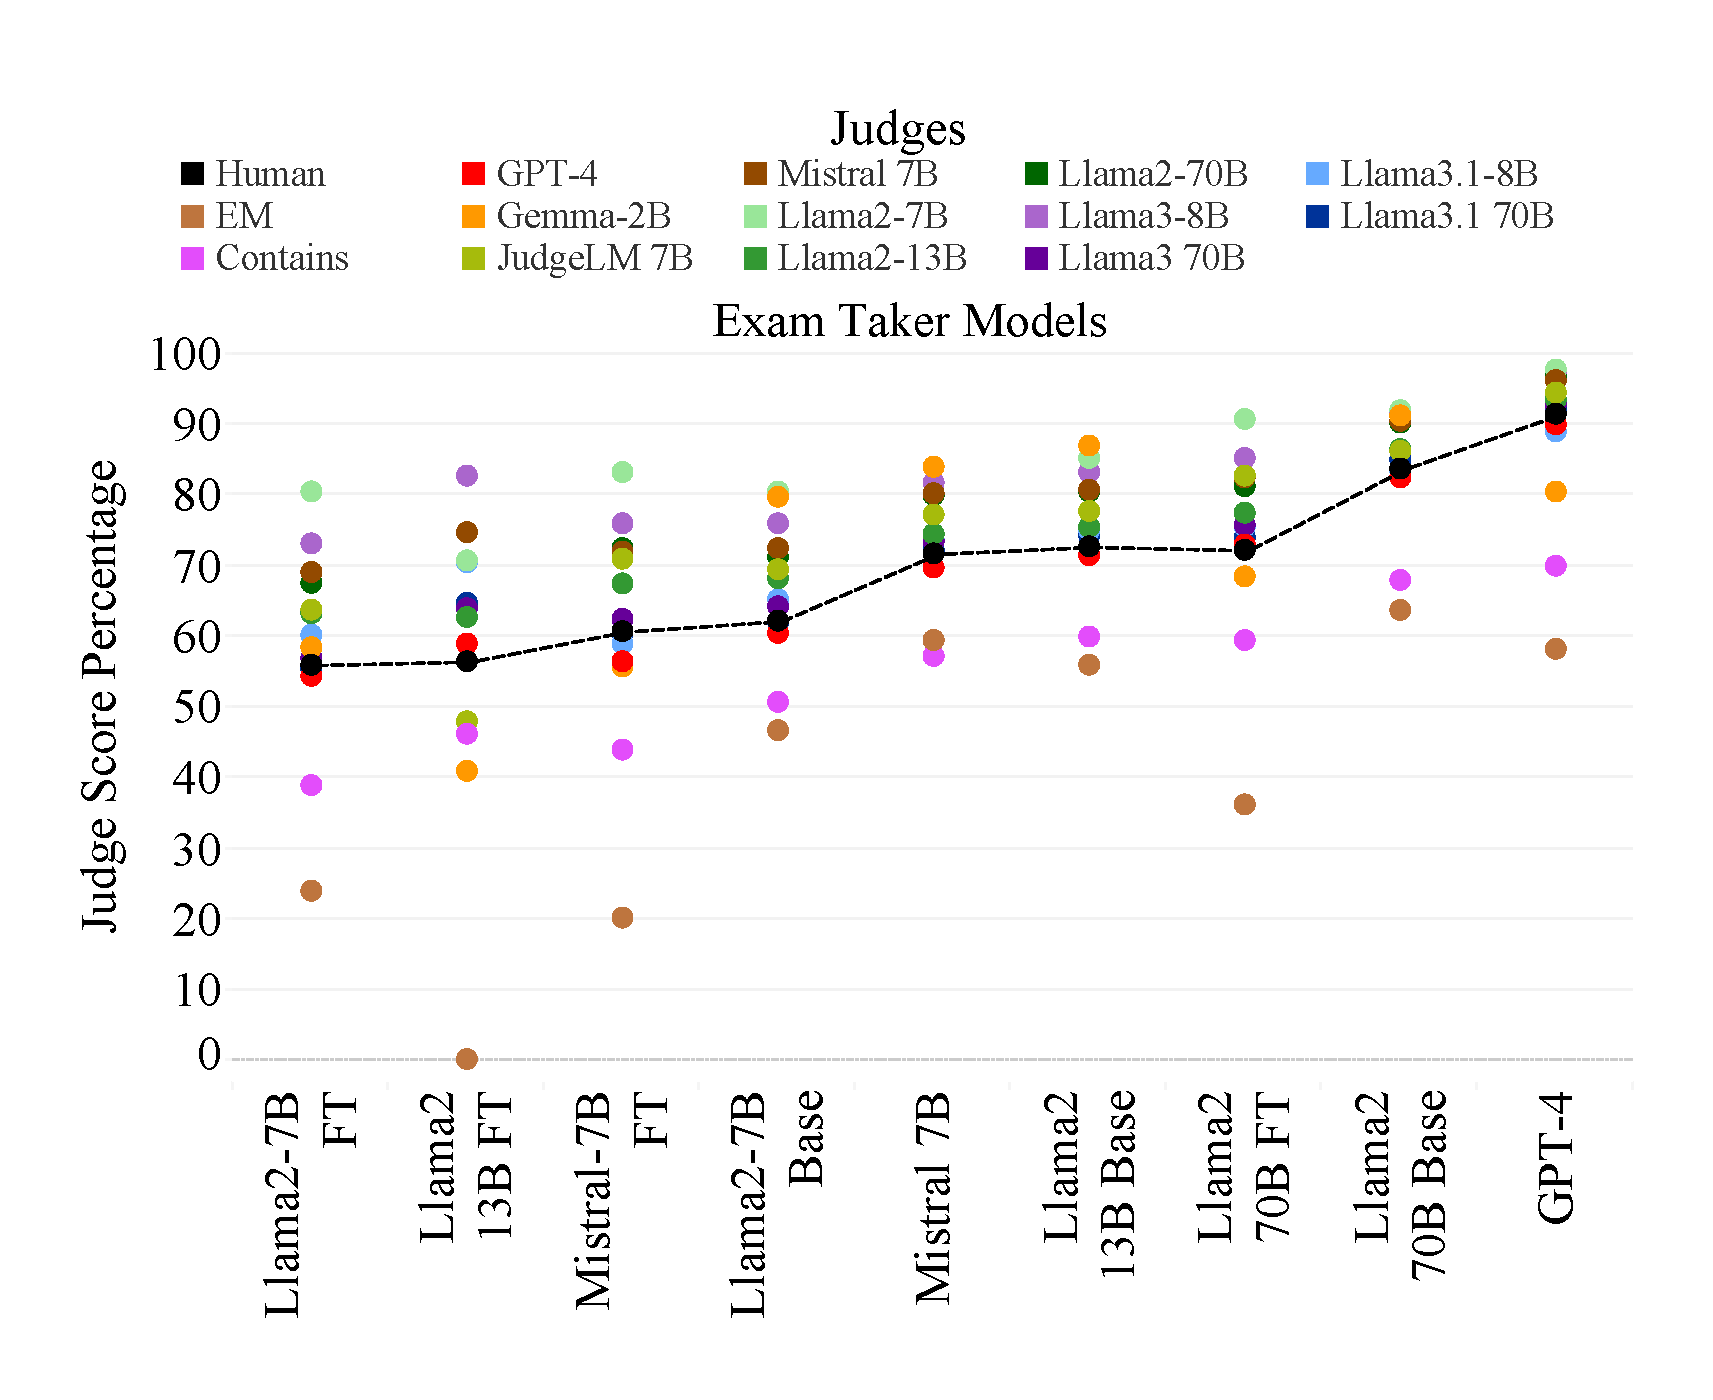
\includegraphics[width=\linewidth]{figures/Scores_HG_V3.pdf}
        \vspace{-6mm}
        \caption{}
        \vspace{-2mm}
        \label{fig:llmalignment_a}
    \end{subfigure}
    \hfill
    \begin{subfigure}[b]{0.44\textwidth}
        \centering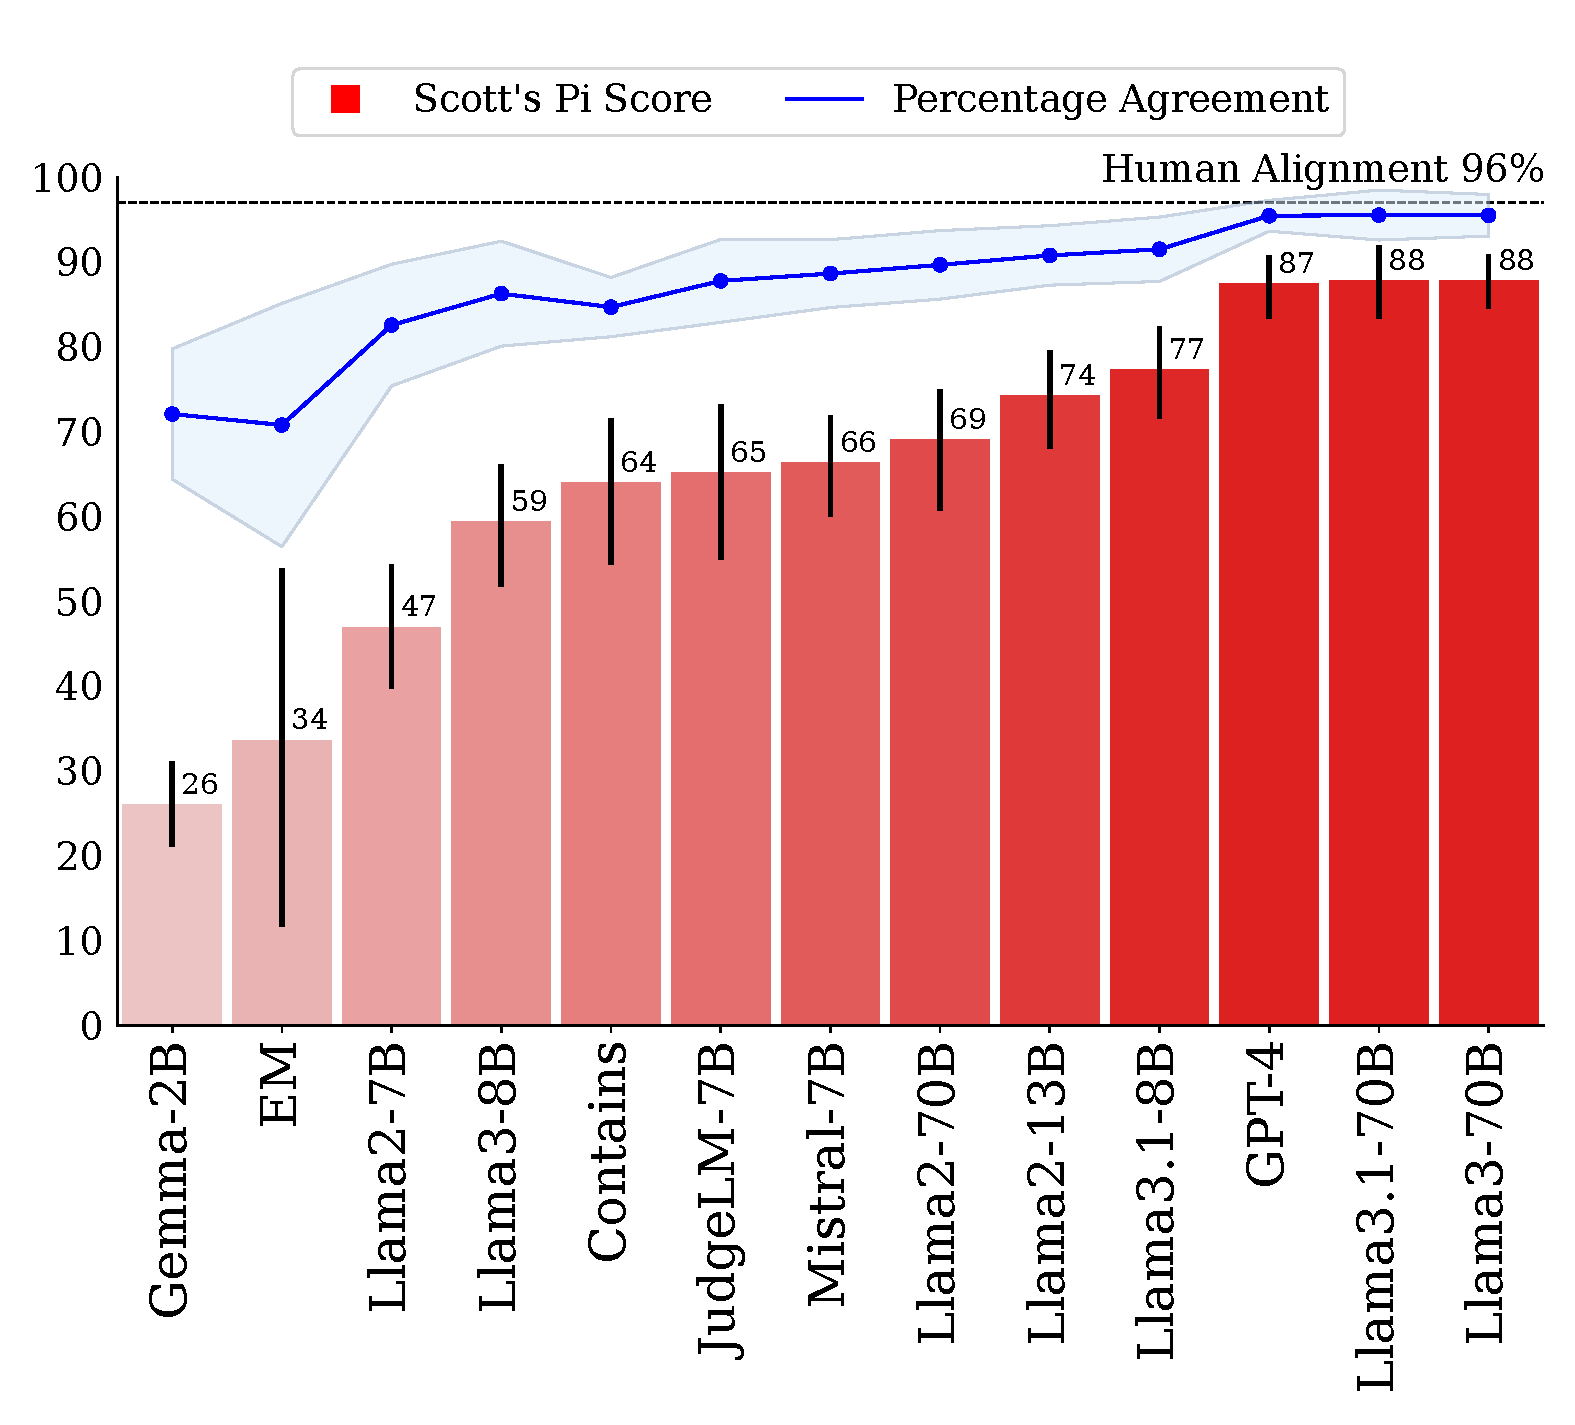
\includegraphics[width=\linewidth, height=6.5cm]{figures/LLMAlignment_HG_V1.pdf}
        \vspace{-6mm}
        \caption{}
        \vspace{-2mm}
        \label{fig:llmalignment_b}
    \end{subfigure}
    \caption{\textbf{Average scores assigned by judge models and alignment with human judges.} (a) Scores assigned to all \evaluatormodels by the various \judgemodels. 
    (b) Average percent agreement (blue line) and Scott's $\pi$ scores (red bars) of \judgemodels with human judges (black line).
    Error bars annotate standard deviation across \evaluatormodels. 
    \judge{Llama3 70B}, \judge{Llama3.1 70B} and \judge{\gpt} have Scott's $\pi$ coefficient that are indicative of excellent alignment, but are still well below the human alignment score. % of 96\%.
    }
    \label{fig:llmalignment}
\end{figure*}

Over the last few years, large language models (LLMs) have demonstrated remarkable capabilities across various domains \citep[i.a.]{radford2019language, brown2020language, achiam2023gpt, meta2024llama3}.
% world knowledge \citep{petroni2019language, razeghi2022impact} and the ability to learn specialized tasks from a few examples \citep{brown2020language}. 
% They have been employed in various tasks including generating free-form responses \citep{}, condensing extensive textual data \citep{pu2023summarization}, conducting search \citep{}, categorizing or grouping documents \citep{}, and facilitating question-answering systems \citep{vectara_llm_use_cases}. 
% 
As more and more new LLMs with different architectures and training methods continue to be released and their capabilities expand, accurately evaluating their performance and limitations becomes increasingly challenging \citep{zheng2024judging,ohmer2024form,benchekroun2023worldsense,madaan2024quantifying,li2023generative}.
% The empirical evaluation of LLMs is particularly difficult due to the diversity of their outputs and the variety of tasks they are used for \citep{li2023generative}. 


LLM evaluation methods generally fall into one of two broad categories. Benchmarks such as MMLU \citep{mmlu}, TruthfulQA \citep{lin2021truthfulqa}, and GSM8K \citep{cobbe2021training} assess specific capabilities, while leaderboards such as Chatbot Arena \citep{chiang2024chatbot} and Open LLM Leaderboard \citep{open-llm-leaderboard} rank models based on human or automated pairwise comparisons. Both approaches face challenges in evaluating free-form text responses, as assessment can be as difficult as generation itself \citep[see e.g.][]{chang2023survey, bavaresco2024llmsinsteadhumanjudges}.

% To evaluate LLMs, various methods have been proposed, typically falling into one of two broad categories. 
% First, benchmarks such as MMLU \citep{mmlu}, TruthfulQA \citep{lin2021truthfulqa}, or GSM8K \citep{cobbe2021training} are used to evaluate specific capabilities of LLMs in an automated manner. 
% Additionally, leaderboards like Chatbot Arena \citep{chiang2024chatbot} and Open LLM Leaderboard \citep{open-llm-leaderboard} assign ranks to models considering pair-wise rankings of LLM outputs, done by humans or, in some cases, automated evaluation methods.
% Since both strategies involve evaluating free-form text responses generated by the LLMs, even in the first case, evaluating the responses is often just as challenging as generating them \citep[see e.g.][]{chang2023survey, bavaresco2024llmsinsteadhumanjudges}. 

One approach to evaluating LLMs is using MCQ benchmarks like MMLU, which compare answer log-probabilities instead of assessing generated responses directly. However, this approach limits the range of measurable abilities and differs from how LLMs are used in practice. Lexical methods, such as exact match (EM) or n-gram overlap, are practical and cost-effective but prone to false negatives and often miss subtle semantic differences. These challenges are amplified for instruction-tuned chat models, which tend to produce more verbose responses \citep{saito2023verbosity, renze2024benefits}.

% One proposed solution to this problem is to use multiple-choice question (MCQ) benchmarks such as MMLU, and compare the log-probabilities of the potential answers rather than evaluating the generated answer directly. 
% However, the MCQ paradigm limits the range of abilities that can be evaluated, and the setup increasingly diverges from how LLMs are used in practice.
% Alternatively, the use of lexical matching methods such as exact match (EM) or n-gram overlap to evaluate the responses are practical and cost-efficient approaches, but are susceptible to false negatives and often fail to adequately distinguish between responses with subtle differences that change their semantic meaning.
% This issue is exacerbated when evaluating instruction-tuned ``chat'' models that are fine-tuned to carry out conversations with humans in natural language, since their responses tend to be more verbose \citep{saito2023verbosity, renze2024benefits}. 
% 
For these reasons, human evaluation remains the gold standard for evaluating LLM responses. %, especially since many benchmarks aim to assess how useful the LLMs are to humans. 

\begin{table*}
    \centering
    \renewcommand{\arraystretch}{1.1} % Increase row height
    \begin{tabular}{|>{\centering\arraybackslash}m{4.5cm}|>{\arraybackslash}m{9cm}|}
        \hline
        \textbf{\Evaluatormodels (base \& instruction-tuned)} & \eval{Llama-2 (7B, 13B, 70B)}, \eval{Mistral 7B}, \eval{\gpt} \\
        \hline
        \textbf{\Judgemodels (instruction-tuned)} & \judge{Llama-2 (7B, 13B, 70B)}, \judge{Llama-3 (8B, 70B)}, \judge{Llama-3.1 (8B, 70B)}, \judge{Gemma 2B}, \judge{Mistral 7B}, \judge{JudgeLM 7B}, \judge{\gpt} \\
        \hline
        \textbf{\Judgemodels (lexical)} & \judge{Exact Match (EM), Contains} \\
        \hline
    \end{tabular}
     \caption{\textbf{\Evaluatormodels and \judgemodels} We consider a wide variety of \evaluatormodels and \judgemodels; to get an in-depth overview of their abilities, we consider \evaluatormodels of various sizes \& types.}
    \label{tab:evaluation}
\end{table*}

Human evaluation is, however, expensive and often impractical, leading to the growing use of LLMs as \judgemodels \citep{lin2021truthfulqa,islam2023financebench,chiang2023can,liusie2024llm}. While promising alignment with humans has been noted \citep{sottana2023evaluation,zheng2024judging}, questions about this approach remain. This work examines LLMs as judges, contrasting them with humans and automated methods. Unlike prior studies, we focus on scenarios with high human alignment to separate task ambiguity from \judgemodel limitations. Using TriviaQA \citep{joshi2017triviaqa}, we evaluate how \textit{\judgemodels} of varying architectures and sizes assess \textit{\evaluatormodels}.

% However, human evaluation is expensive, time-consuming, and often impractical in many use cases. 
% As a result, it has increasingly become common practice to evaluate LLM responses using another LLM as a \judgemodel \citep{lin2021truthfulqa,islam2023financebench,chiang2023can,liusie2024llm}.
% While there are promises of alignment between LLM judges and humans \citep{sottana2023evaluation,zheng2024judging}, there are also many open questions about the strengths and weaknesses of the paradigm.
% 
In this work, we study the properties of LLMs as judges, comparing them with humans and automated evaluation methods.
Contrary to prior work, we focus on a clean scenario in which human alignment is very high, 
allowing us to distinguish ambiguity and subjectivity in the task itself from potential issues with the \judgemodels.
Using the knowledge benchmark TriviaQA \citep{joshi2017triviaqa} as our playground, we investigate how \njudgesword different \textit{\judgemodels} with varying architectures and sizes judge \nexamtakersword different \textit{\evaluatormodels}.
% Our main findings are:\begin{itemize}[wide, labelwidth=2pt, labelindent=2pt]\setlength\itemsep{1em}
    Our main findings are:
    % \vspace{-1mm}
% \begin{itemize}[wide, labelwidth=2pt, labelindent=2pt,topsep=-4pt, itemsep=-2pt]%\setlength\itemsep{1em}
\begin{itemize}[leftmargin=4pt, topsep=1pt, itemsep=0.1em] %\setlength\itemsep{0.1em}
    \item \textbf{Even in clean setups, only the best models have high alignment scores}. Among the \njudgesword \judgemodels, only \judge{\gpt}, \judge{Llama-3.1;70B}, and \judge{Llama-3;70B} achieved strong alignment with humans. However, even these fall short of the human alignment coefficient (\cref{fig:llmalignment}). %\vspace{-1mm}
% \item While previous work commonly used percent agreement, \textbf{Cohen's kappa distinguishes judges much better}, since in some cases, high percent agreement can still give very divergent scores (\cref{fig:cohenskappa}).
\\
\item \textbf{\scottspi distinguishes judges better than percent alignment}. In terms of percent alignment, judges are rarely discriminable, while \scottspi provides a more informative signal. In some cases, high percent agreement can still give scores that differ 10-20 points from the human-assigned scores (\cref{fig:alignment_vs_delta}). %\vspace{-0.5mm}

\item \textbf{Also \scottspi is not all telling} While \judge{\gpt} and \judge{Llama-3} achieve excellent alignment scores, they can differ by up to 5 points from human scores. Moreover, in discriminating between \evaluatormodels, their performance is comparable to cheaper alternatives like \judge{Mistral 7B} and \judge{contains}, which have lower alignment scores but more consistent biases (\cref{fig:ranking_posneg}).

% \item \textbf{Also \scottspi is not all telling}. While \judge{\gpt} and \judge{Llama-3} both have alignment scores that are considered excellent, their scores still differ up to 5 points from human-assigned scores. Furthermore, when it comes to \textit{discriminating} different \evaluatormodels, their results are comparable to alternative cheaper approaches such as \judge{Mistral\;7B} and \judge{contains}, which have much lower alignment scores but more consistent biases (\cref{fig:ranking_posneg}).

\end{itemize}

Through detailed analysis (\cref{sec:analysis}), we gain insights into judge performance. Improved alignment appear to be driven from higher recall rates and fewer false negatives. However, \judgemodels struggle with under-specified answers and exhibit leniency, reducing evaluation consistency. They are also sensitive to prompt length and quality. Surprisingly, even when asked to evaluate a verbatim match with a reference, \judgemodels sometimes fail.

Overall, our work highlights the strengths of the LLM-as-a-judge paradigm, while cautioning against overreliance on alignment metrics, even when they are high. Through error analysis, we identify common failure cases, contributing to a deeper understanding of this emerging evaluation paradigm. With this work, our objective is to improve understanding of the emerging mainstream paradigm for evaluating LLM.

% Through detailed analysis (\cref{sec:analysis}), we uncover additional insights into judge performance. 
% Improved alignment appears to be driven by improved recall rates and reduced false negatives. 
% However, \judgemodels struggle with under-specified answers and tend to be lenient, affecting their evaluation consistency. 
% They are also sensitive to the length and quality of prompts.
% And, surprisingly, even when the \judgemodels are asked to evaluate an answer matching verbatim with a reference answer, many \judgemodels still sometimes fail to evaluate it correctly.

% Overall, our work showcases the strengths of the LLM-as-a-judge paradigm while also highlighting the need for caution against overreliance on alignment metrics, even in cases where they are high.

% Through error analysis, we also highlight several common failure cases that require attention.
% With this, we aim to contribute to a better general understanding of what is now becoming a mainstream paradigm for evaluating LLMs.

